\RequirePackage{luatex85}
\documentclass[tikz]{standalone}
% Default preamble
\usepackage{pgfplots}
\pgfplotsset{compat=newest}
\usepgfplotslibrary{groupplots}
\usepgfplotslibrary{polar}
\usepgfplotslibrary{smithchart}
\usepgfplotslibrary{statistics}
\usepgfplotslibrary{dateplot}
\usepgfplotslibrary{ternary}
\begin{document}
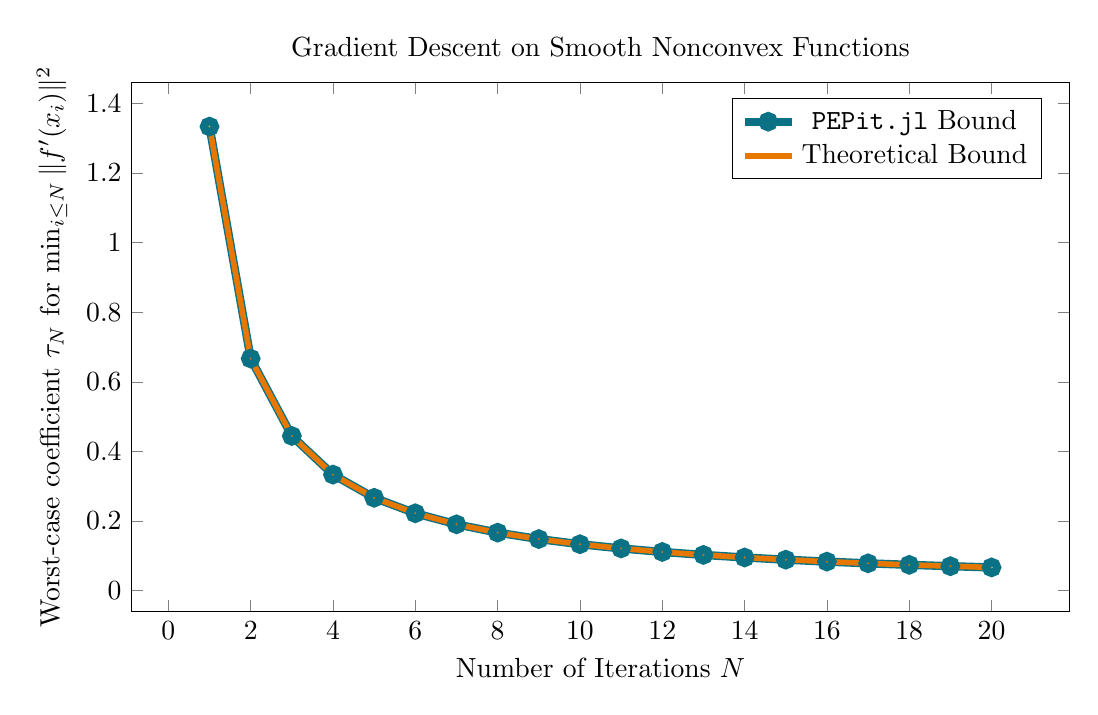
\begin{tikzpicture}
\begin{axis}[width={13.5cm}, height={8.3cm}, title={Gradient Descent on Smooth Nonconvex Functions}, xlabel={Number of Iterations $N$}, ylabel={Worst-case coefficient $\tau_N$ for $\min_{i\leq N}\|f'(x_i)\|^2$}, legend pos={north east}, axis lines={box}]
    \addplot+[color={{rgb,255:red,11;green,114;blue,133}}, mark={o}, line width={3pt}]
        coordinates {
            (1,1.3333333328709172)
            (2,0.6666666662974063)
            (3,0.44444444407435413)
            (4,0.3333333306865022)
            (5,0.26666666653052024)
            (6,0.22222222162442798)
            (7,0.1904761904489271)
            (8,0.16666666654511467)
            (9,0.14814814756265404)
            (10,0.13333333329451558)
            (11,0.1212121211195289)
            (12,0.11111111097689964)
            (13,0.10256410240920882)
            (14,0.09523809509712118)
            (15,0.08888888832147421)
            (16,0.0833333328170411)
            (17,0.07843137253193336)
            (18,0.07407407401594858)
            (19,0.07017543849705375)
            (20,0.06666666624383845)
        }
        ;
    \addlegendentry {$\texttt{PEPit.jl}$ Bound}
    \addplot+[color={{rgb,255:red,230;green,119;blue,0}}, no marks, line width={2pt}]
        coordinates {
            (1,1.3333333333333333)
            (2,0.6666666666666666)
            (3,0.4444444444444444)
            (4,0.3333333333333333)
            (5,0.26666666666666666)
            (6,0.2222222222222222)
            (7,0.19047619047619047)
            (8,0.16666666666666666)
            (9,0.14814814814814814)
            (10,0.13333333333333333)
            (11,0.1212121212121212)
            (12,0.1111111111111111)
            (13,0.10256410256410256)
            (14,0.09523809523809523)
            (15,0.08888888888888888)
            (16,0.08333333333333333)
            (17,0.0784313725490196)
            (18,0.07407407407407407)
            (19,0.07017543859649122)
            (20,0.06666666666666667)
        }
        ;
    \addlegendentry {$\textrm{Theoretical Bound}$}
\end{axis}
\end{tikzpicture}
\end{document}
